\cleardoublepage



\chapter{Étude de fonctionnement}

La première partie de notre projet a consisté à étudier les différentes étapes du fonctionnement de notre solution : de la réception d'un SMS sur le smartphone à son affichage sur le PC, mais aussi de l'écriture d'un message sur le PC jusqu'à son envoi par le smartphone.
Nous détaillerons plus précisément le choix du service proposé à l'utilisateur pour l'envoi du SMS depuis l'ordinateur.
\\





%%%%%%%%%%%%%%%%%%%%%%%%%%%%%%%%%%%%%%%%%%%%%%%%%%%%%%%%%%%%%%%%%%%%%%%%%%%%%%%%%%%%%%%%%%%%%%%%%%%%
%%%%%%%%%%%%%%%%%%%%%%%%%%%%%%%%%%%%%%%%%%%%%%%%%%%%%%%%%%%%%%%%%%%%%%%%%%%%%%%%%%%%%%%%%%%%%%%%%%%%
%%%%%%%%%%%%%%%%%%%%%%%%%%%%%%%%%%%%%%%%%%%%%%%%%%%%%%%%%%%%%%%%%%%%%%%%%%%%%%%%%%%%%%%%%%%%%%%%%%%%
%%%%%%%%%%%%%%%%%%%%%%%%%%%%%%%%%%%%%%%%%%%%%%%%%%%%%%%%%%%%%%%%%%%%%%%%%%%%%%%%%%%%%%%%%%%%%%%%%%%%
%%%%%%%%%%%%%%%%%%%%%%%%%%%%%%%%%%%%%%%%%%%%%%%%%%%%%%%%%%%%%%%%%%%%%%%%%%%%%%%%%%%%%%%%%%%%%%%%%%%%

\section{Transfert du message}

%%%%%%%%%%%%%%%%%%%%%%%%%%%%%%%%%%%%%%%%%%%%%%%%%%%%%%%%%%%%%%%%%%%%%%%%%%%%%%%%%%%%%%%%%%%%%%%%%%%%
%%%%%%%%%%%%%%%%%%%%%%%%%%%%%%%%%%%%%%%%%%%%%%%%%%%%%%%%%%%%%%%%%%%%%%%%%%%%%%%%%%%%%%%%%%%%%%%%%%%%
%%%%%%%%%%%%%%%%%%%%%%%%%%%%%%%%%%%%%%%%%%%%%%%%%%%%%%%%%%%%%%%%%%%%%%%%%%%%%%%%%%%%%%%%%%%%%%%%%%%%

\subsection{Protocole XMPP}

%%%%%%%%%%%%%%%%%%%%%%%%%%%%%%%%%%%%%%%%%%%%%%%%%%%%%%%%%%%%%%%%%%%%%%%%%%%%%%%%%%%%%%%%%%%%%%%%%%%%

\subsubsection{Présentation}

\textit{Jabber}, maintenant appelé \textit{XMPP}\footnote{Site web : \href{http://xmpp.org/}{http://xmpp.org/}} (eXtensible Messaging and Presence Protocol) suite à sa standardisation, est un protocole de messagerie instantanée et de présence sur internet.
Bien que peu connu du public, ce protocole possède de très nombreux avantages :
\begin{itemize}
	\item standard ouvert : son fonctionnement est accessible par tous ;
	\item simple d'utilisation : les clients XMPP sont très simple d'utilisation car toute la complexité du protocole est situé coté serveur ;
	\item décentralisé ;
	\item confidentialité et sécurité ;
	\item ...
\\
\end{itemize}

Le protocole XMPP est de plus en plus utilisé par les services de messagerie instantanée, tels que iChat sur les produits Apple, le chat Facebook, ou Gtalk de Google que nous utiliserons dans ce projet.
\\

%%%%%%%%%%%%%%%%%%%%%%%%%%%%%%%%%%%%%%%%%%%%%%%%%%%%%%%%%%%%%%%%%%%%%%%%%%%%%%%%%%%%%%%%%%%%%%%%%%%%

\subsubsection{Bibliothèques}

En raison de la nature dynamique, évolutive et ouverte du protocole XMPP, de très nombreuses bibliothèques sont disponibles (référencées sur le \href{http://xmpp.org/xmpp-software/libraries/}{site officiel} de la fondation) dans la majorité des langages de programmation.

Dans ce projet nous utiliserons aSmack, un portage sous Androïd de Smack, une bibliothèque Java, ainsi que XMPPFramework une bibliothèque pour Objective-C.
\\



%%%%%%%%%%%%%%%%%%%%%%%%%%%%%%%%%%%%%%%%%%%%%%%%%%%%%%%%%%%%%%%%%%%%%%%%%%%%%%%%%%%%%%%%%%%%%%%%%%%%
%%%%%%%%%%%%%%%%%%%%%%%%%%%%%%%%%%%%%%%%%%%%%%%%%%%%%%%%%%%%%%%%%%%%%%%%%%%%%%%%%%%%%%%%%%%%%%%%%%%%
%%%%%%%%%%%%%%%%%%%%%%%%%%%%%%%%%%%%%%%%%%%%%%%%%%%%%%%%%%%%%%%%%%%%%%%%%%%%%%%%%%%%%%%%%%%%%%%%%%%%

\subsection{Choix du protocole}

La première raison qui nous a poussé à choisir le protocole XMPP pour échanger les messages entre l'ordinateur et le smartphone est le fait qu'il s'agit du protocole de base de GTalk.
A l'origine nous voulions envoyer et recevoir les messages depuis GTalk.
Nous vous expliquerons dans la partie \ref{Service proposé} les détails du service que nous proposerons à l'utilisateur.
\\





%%%%%%%%%%%%%%%%%%%%%%%%%%%%%%%%%%%%%%%%%%%%%%%%%%%%%%%%%%%%%%%%%%%%%%%%%%%%%%%%%%%%%%%%%%%%%%%%%%%%
%%%%%%%%%%%%%%%%%%%%%%%%%%%%%%%%%%%%%%%%%%%%%%%%%%%%%%%%%%%%%%%%%%%%%%%%%%%%%%%%%%%%%%%%%%%%%%%%%%%%
%%%%%%%%%%%%%%%%%%%%%%%%%%%%%%%%%%%%%%%%%%%%%%%%%%%%%%%%%%%%%%%%%%%%%%%%%%%%%%%%%%%%%%%%%%%%%%%%%%%%
%%%%%%%%%%%%%%%%%%%%%%%%%%%%%%%%%%%%%%%%%%%%%%%%%%%%%%%%%%%%%%%%%%%%%%%%%%%%%%%%%%%%%%%%%%%%%%%%%%%%
%%%%%%%%%%%%%%%%%%%%%%%%%%%%%%%%%%%%%%%%%%%%%%%%%%%%%%%%%%%%%%%%%%%%%%%%%%%%%%%%%%%%%%%%%%%%%%%%%%%%

\section{Service proposé}
\label{Service proposé}

%%%%%%%%%%%%%%%%%%%%%%%%%%%%%%%%%%%%%%%%%%%%%%%%%%%%%%%%%%%%%%%%%%%%%%%%%%%%%%%%%%%%%%%%%%%%%%%%%%%%
%%%%%%%%%%%%%%%%%%%%%%%%%%%%%%%%%%%%%%%%%%%%%%%%%%%%%%%%%%%%%%%%%%%%%%%%%%%%%%%%%%%%%%%%%%%%%%%%%%%%
%%%%%%%%%%%%%%%%%%%%%%%%%%%%%%%%%%%%%%%%%%%%%%%%%%%%%%%%%%%%%%%%%%%%%%%%%%%%%%%%%%%%%%%%%%%%%%%%%%%%

\subsection{GTalk}

Google Talk, aussi appelé GTalk, est le client de messagerie instantanée proposé par Google.
Il est disponible à partir de la page web de Gmail, mais aussi en cleint Windows que l'on peut installer sur son ordinateur.

A l'origine nous voulions utiliser ce client pour envoyer nos SMS pour la simple et bonne raison que de nombreux utilisateurs ont toujours le navigateur web ouvert, ainsi qu'un onglet avec leur boite mail.
\\

%%%%%%%%%%%%%%%%%%%%%%%%%%%%%%%%%%%%%%%%%%%%%%%%%%%%%%%%%%%%%%%%%%%%%%%%%%%%%%%%%%%%%%%%%%%%%%%%%%%%

\subsubsection{Parler à soi-même}

Le protocole XMPP autorise et offre la possibilité de s'envoyer des messages instantanés à soi-même, si l'expéditeur et le destinataire sont les mêmes comptes.

Cependant GTalk ne le permet pas, pour au moins deux raisons :
\begin{itemize}
	\item Pour envoyer un message à une personne il faut cliquer sur son lien dans la liste des contacts ;
	Or notre propre adresse email n'y apparait pas même si l'on s'est ajouté dans nos contacts.
	\item Gtalk n'affiche pas les messages que l'on s'envoie à soi-même, depuis un autre client XMPP, comme une application mobile par exemple.
\end{itemize}

De ce fait il est donc nécessaire d'utiliser un compte intermédiaire.
On peut ainsi créer un compte spécial qui représenterai notre smartphone, et qui sera utilisé uniquement par l'application.
\\

%%%%%%%%%%%%%%%%%%%%%%%%%%%%%%%%%%%%%%%%%%%%%%%%%%%%%%%%%%%%%%%%%%%%%%%%%%%%%%%%%%%%%%%%%%%%%%%%%%%%

\subsubsection{Praticité}

Notre première solution envisagée consistait à envoyer le message depuis GTalk, en tapant par exemple :
\begin{lstlisting}
sms 0123456789 Coucou, comment vas-tu ?
\end{lstlisting}
~~\\

Cette méthode pose toutefois plusieurs inconvénients :
\begin{itemize}
	\item Le message doit être formaté correctement par l'utilisateur pour pouvoir être traité ;
	\item Il est nécessaire de connaitre le numéro de téléphone du destinataire pour pouvoir envoyer le message.
\end{itemize}
~~\\



%%%%%%%%%%%%%%%%%%%%%%%%%%%%%%%%%%%%%%%%%%%%%%%%%%%%%%%%%%%%%%%%%%%%%%%%%%%%%%%%%%%%%%%%%%%%%%%%%%%%
%%%%%%%%%%%%%%%%%%%%%%%%%%%%%%%%%%%%%%%%%%%%%%%%%%%%%%%%%%%%%%%%%%%%%%%%%%%%%%%%%%%%%%%%%%%%%%%%%%%%
%%%%%%%%%%%%%%%%%%%%%%%%%%%%%%%%%%%%%%%%%%%%%%%%%%%%%%%%%%%%%%%%%%%%%%%%%%%%%%%%%%%%%%%%%%%%%%%%%%%%

\subsection{Solution envisagée}

Suite aux inconvénients de GTalk mentionnés précédemment, nous nous sommes orientés vers un site web qui permettrait une utilisation plus intuitive et pratique pour l'utilisateur.
\\

Malgré le fait qu'il faille se connecter un site tiers, cette solution permet de résoudre les différents problèmes :
\begin{itemize}
	\item Grâce à une bibliothèque fournie par Google il est possible d'accéder aux contacts depuis notre site web, ce qui évite de devoir spécifier le numéro du destinataire ;
	\item Le site s'occupe de formater le message XMPP envoyé entre le PC et l'application du smartphone ;
	\item L'utilisateur n'a pas besoin de créer un nouveau compte pour pouvoir utiliser notre solution.
\\
\end{itemize}

\begin{figure}[!h]
	\center
	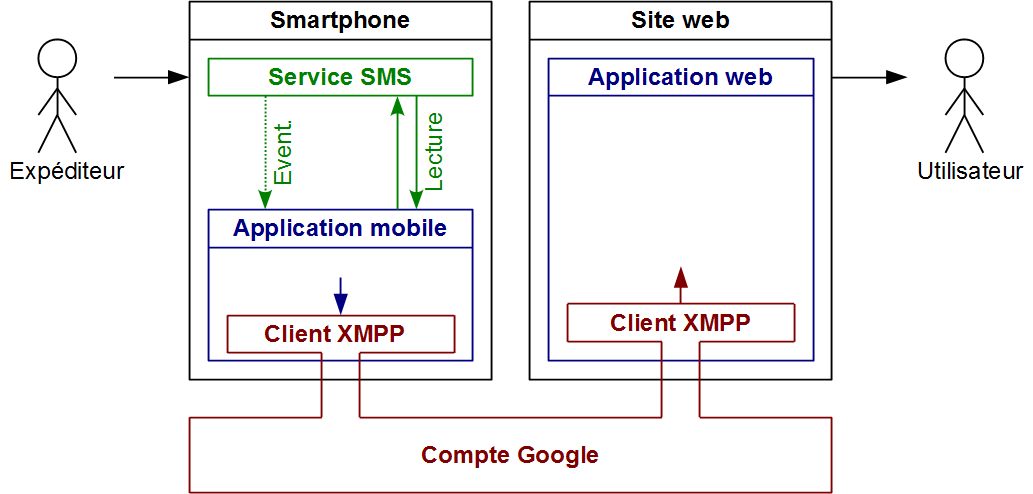
\includegraphics[scale=0.5]{img/schemaFonctionnement_siteWeb_reception.png}
	\caption{Site web : Réception d'un SMS}
	\label{schemaFonctionnement_siteWeb_reception}
\end{figure}
Le schéma \ref{schemaFonctionnement_siteWeb_reception} représente les différentes étapes de notre solution :
\begin{enumerate}
	\item Le smartphone reçoit un SMS de la part du destinataire ;
	\item L'application mobile reçoit un événement indiquant la réception d'un nouveau SMS ;
	\item L'application mobile lit le SMS : le numéro de téléphone du destinataire + le contenu du SMS ;
	\item L'application mobile envoie un message XMPP (formaté pour pouvoir être traité) au propre compte Google de l'utilisateur ;
	\item Le client XMPP de l'application web reçoit le message XMPP ;
	\item L'application web analyse le message XMPP puis affiche le SMS à l'utilisateur.
\end{enumerate}